%!TEX root = ../main.tex

\begin{frame}{Resultados Finais}
 \begin{itemize}
   \item Utilização de um servidor para treinamento das CNNs:
    \begin{itemize}
      \item Processador Intel Core i7
      \item 16 GB de RAM
      \item GPU Nvidia GeForce GTX 1080 com 11 GB de memória
    \end{itemize}
    \bigskip
    \item Modelos degenerados tiveram seus resultados descartados
    \begin{itemize}
      \item \emph{Dying ReLU problem}
      \item Permanência em mínimos locais no treinamento
    \end{itemize}
   \end{itemize}
\end{frame}

\begin{frame}{LeNet}

  \begin{table}[h]
    \centering
    \caption{Detalhamento dos melhores resultados obtidos com a arquitetura LeNet.}
    \label{tab:lenet}
    \resizebox{\textwidth}{!}{\begin{tabular}{ccccccc}
    \toprule
    \textbf{Abordagem} & \textbf{Otimizador} & \textbf{\emph{Patience}}  & \textbf{Função de Ativação} & \textbf{Acurácia} & \textbf{\emph{F-Score}} & \textbf{EER} \\
    \midrule
    Abordagem A & RMSprop & 5 & ReLU & $0.9865$ & $0.9755$ & $1.1679$\\
    Abordagem B & Adam & 10 & ELU & $0.8361$ & $0.8159$ & $12.5245$ \\
    \bottomrule
    \end{tabular}}
    \end{table}

\end{frame}

\begin{frame}{LeNet}

  \begin{figure}[h!]
    \centering
    \caption{Histórico de \emph{loss} e acurácia durante o treinamento dos melhores modelos obtidos com a arquitetura LeNet.}
    \begin{subfigure}{0.3\linewidth}
      \caption{\emph{Loss} LeNet A.\label{subfig:lenet-a-loss}}
      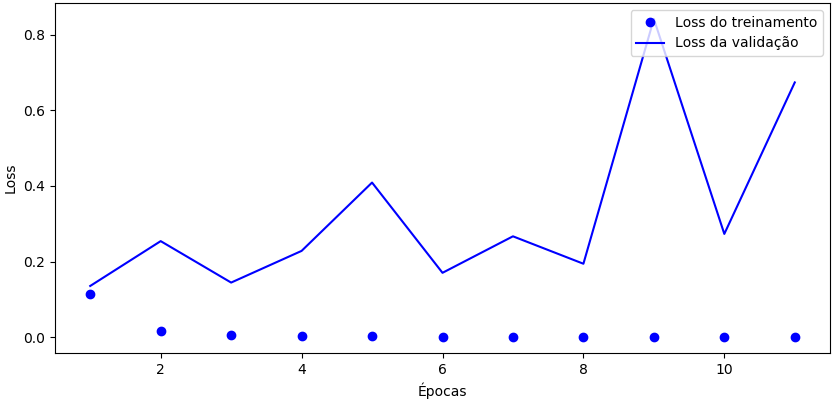
\includegraphics[width=\linewidth]{img/lenet-a-loss}%
    \end{subfigure}
    \hspace{1.5cm}
    \begin{subfigure}{0.3\linewidth}
      \caption{Acurácia LeNet A.\label{subfig:lenet-a-acc}}
      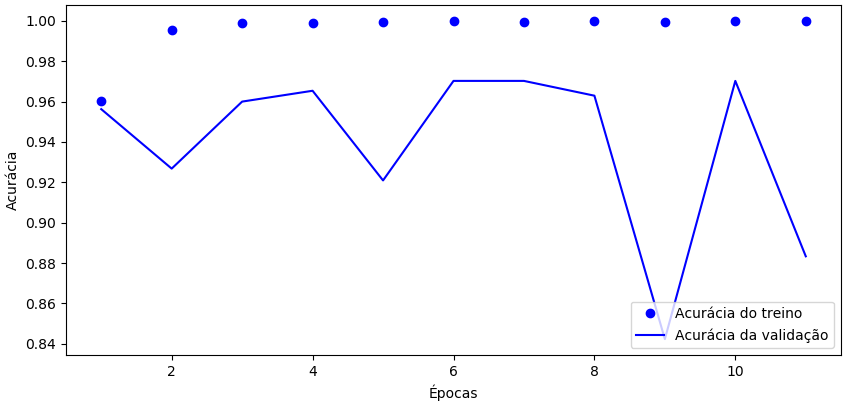
\includegraphics[width=\linewidth]{img/lenet-a-acc}%
    \end{subfigure}
    \hspace{1.5cm}
    \begin{subfigure}{0.3\linewidth}
      \caption{\emph{Loss} LeNet B.\label{subfig:lenet-b-loss}}
      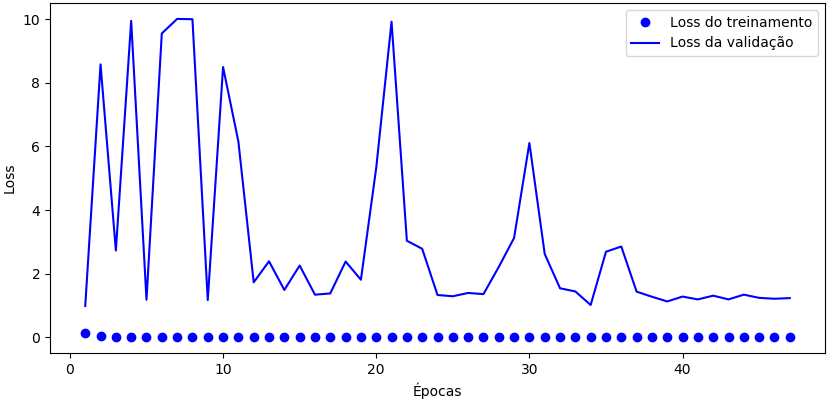
\includegraphics[width=\linewidth]{img/lenet-b-loss}%
    \end{subfigure}
    \hspace{1.5cm}
    \begin{subfigure}{0.3\linewidth}
      \caption{Acurácia LeNet B.\label{subfig:lenet-b-acc}}
      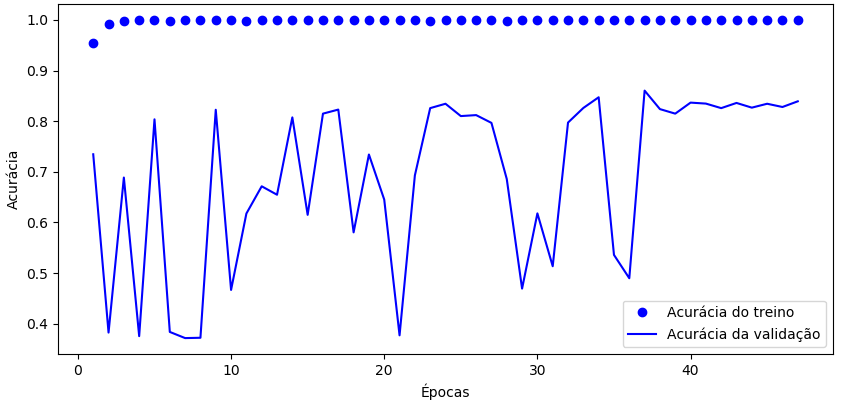
\includegraphics[width=\linewidth]{img/lenet-b-acc}%
    \end{subfigure}
    \label{fig:treinamento-lenet}
  \end{figure}

\end{frame}

\begin{frame}{LeNet}
  \vskip1\baselineskip
  \begin{figure}[ht!]
      \caption{Matrizes de confusão dos melhores modelos obtidos com a arquitetura LeNet.}\label{fig:matrizes-lenet}
      \begin{subfigure}{0.4\linewidth}
        \caption{LeNet A}
        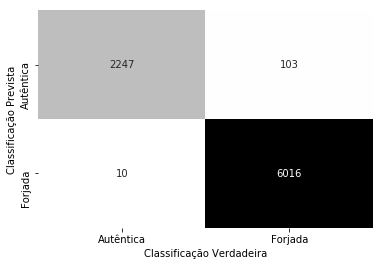
\includegraphics[width=\linewidth]{img/matriz-lenet-a}
      \end{subfigure}
      \hspace{2cm}
      \begin{subfigure}{0.4\linewidth}
        \caption{LeNet B}
        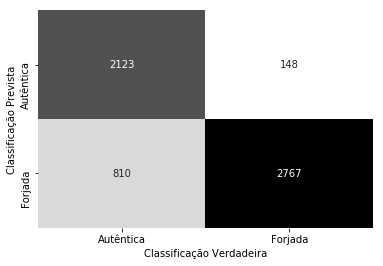
\includegraphics[width=\linewidth]{img/matriz-lenet-b}%
      \end{subfigure}
  \end{figure}
\end{frame}


\begin{frame}{AlexNet}

  \begin{table}[h!]
    \centering
    \caption{Detalhamento dos melhores modelos obtidos com a arquitetura AlexNet para cada uma das abordagens consideradas neste trabalho.}
    \label{tab:alexnet}
    \resizebox{\textwidth}{!}{\begin{tabular}{ccccccc}
    \toprule
    \textbf{Abordagem} & \textbf{Otimizador} & \textbf{\emph{Patience}}  & \textbf{Função de Ativação} & \textbf{Acurácia} & \textbf{F-Score} & \textbf{EER} \\
    \midrule
    Abordagem A & Adam & 15 & ELU & $0.9654$ & $0.9393$ & $1.5401$\\
    Abordagem B & RMSprop & 5 & ELU & $0.8593$ & $0.7993$ & $13.8265$\\
    \bottomrule
    \end{tabular}}
    \end{table}

\end{frame}

\begin{frame}{AlexNet}

  \begin{figure}[h!]
    \centering
    \caption{Histórico de \emph{loss} e acurácia durante o treinamento dos melhores modelos obtidos com a arquitetura AlexNet.}
    \begin{subfigure}{0.3\linewidth}
      \caption{\emph{Loss} AlexNet A.\label{subfig:alexnet-a-loss}}
      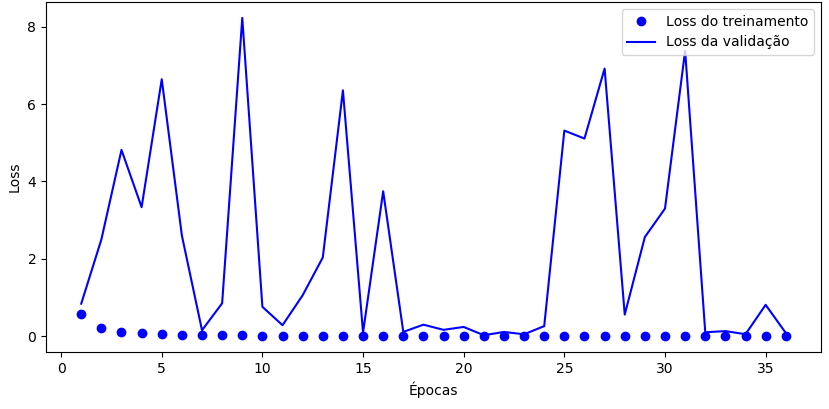
\includegraphics[width=\linewidth]{img/alexnet-a-loss}%
    \end{subfigure}
    \hspace{1.5cm}
    \begin{subfigure}{0.3\linewidth}
      \caption{Acurácia AlexNet A.\label{subfig:alexnet-a-acc}}
      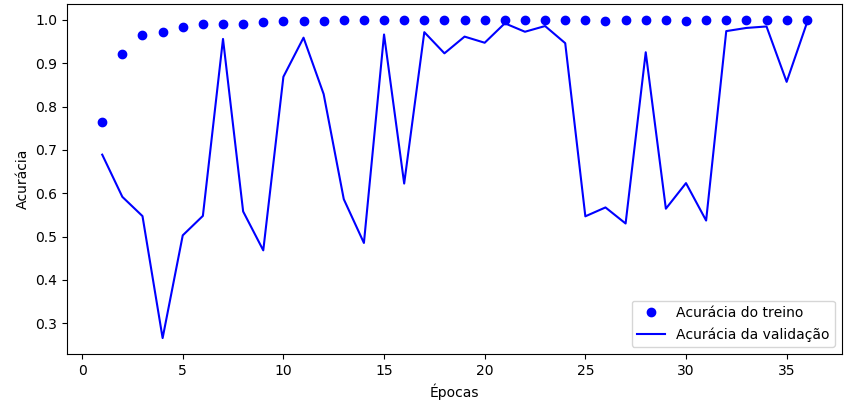
\includegraphics[width=\linewidth]{img/alexnet-a-acc}%
    \end{subfigure}
    \hspace{1.5cm}
    \begin{subfigure}{0.3\linewidth}
      \caption{\emph{Loss} AlexNet B.\label{subfig:alexnet-b-loss}}
      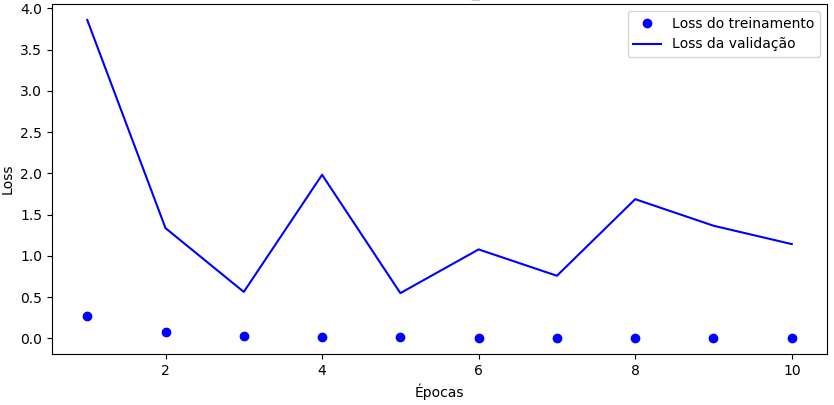
\includegraphics[width=\linewidth]{img/alexnet-b-loss}%
    \end{subfigure}
    \hspace{1.5cm}
    \begin{subfigure}{0.3\linewidth}
      \caption{Acurácia AlexNet B.\label{subfig:alexnet-b-acc}}
      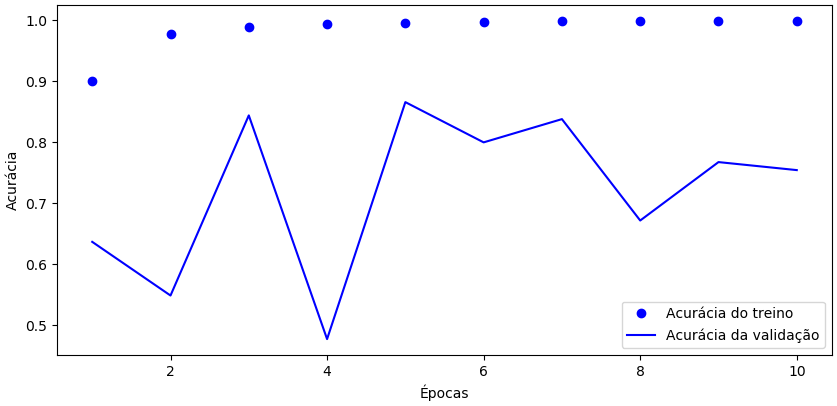
\includegraphics[width=\linewidth]{img/alexnet-b-acc}%
    \end{subfigure}
    \label{fig:treinamento-alexnet}
  \end{figure}
\end{frame}

\begin{frame}{AlexNet}
  \vskip1\baselineskip
  \begin{figure}[ht!]
    \caption{Matrizes de confusão dos melhores modelos obtidos com a arquitetura AlexNet.}\label{fig:matrizes-lenet}
    \begin{subfigure}{0.4\linewidth}
      \caption{AlexNet A}
      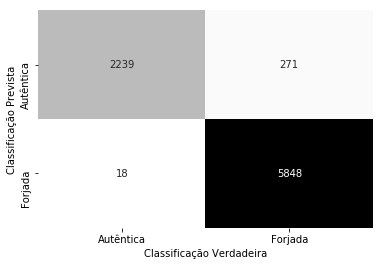
\includegraphics[width=\linewidth]{img/matriz-alexnet-a}
    \end{subfigure}
    \hspace{2cm}
    \begin{subfigure}{0.4\linewidth}
      \caption{AlexNet B}
      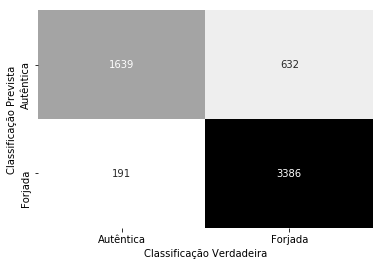
\includegraphics[width=\linewidth]{img/matriz-alexnet-b}%
    \end{subfigure}
\end{figure}
\end{frame}

\begin{frame}{MobileNet}

  \begin{table}[h!]
    \centering
    \caption{Detalhamento dos melhores modelos obtidos com a arquitetura MobileNet para cada uma das abordagens consideradas neste trabalho.}
    \label{tab:mobilenet}
    \resizebox{\textwidth}{!}{\begin{tabular}{ccccccc}
    \toprule
    \textbf{Abordagem} & \textbf{Otimizador} & \textbf{\emph{Patience}}  & \textbf{Função de Ativação} & \textbf{Acurácia} & \textbf{F-Score} & \textbf{EER} \\
    \midrule
    Abordagem A & SGD & 15 & ReLU & $0.9606$ & $0.9318$ & $0.9304$ \\
    Abordagem B & Adam & 15 & ReLU & $0.8856$ & $0.8658$ & $9.9475$\\
    \bottomrule
    \end{tabular}}
    \end{table}

\end{frame}

\begin{frame}{MobileNet}

  \begin{figure}[h!]
    \centering
    \caption{Histórico de \emph{loss} e acurácia durante o treinamento dos melhores modelos obtidos com a arquitetura MobileNet.}
    \begin{subfigure}{0.3\linewidth}
      \caption{\emph{Loss} MobileNet A.\label{subfig:alexnet-a-loss}}
      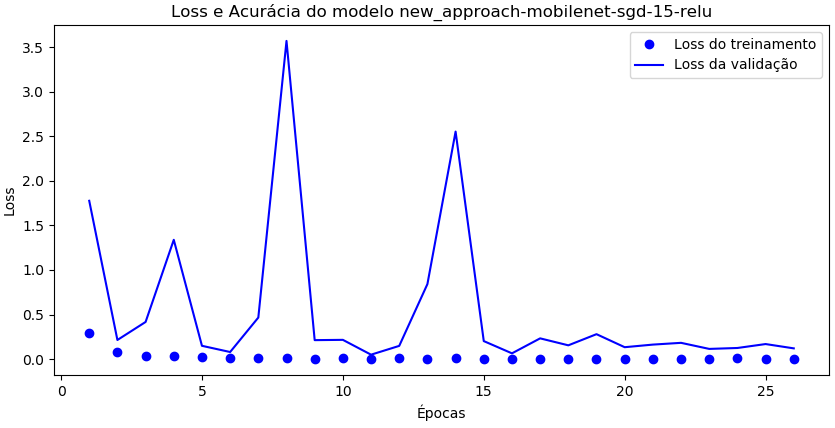
\includegraphics[width=\linewidth]{img/mobilenet-a-loss}%
    \end{subfigure}
    \hspace{1.5cm}
    \begin{subfigure}{0.3\linewidth}
      \caption{Acurácia MobileNet A.\label{subfig:alexnet-a-acc}}
      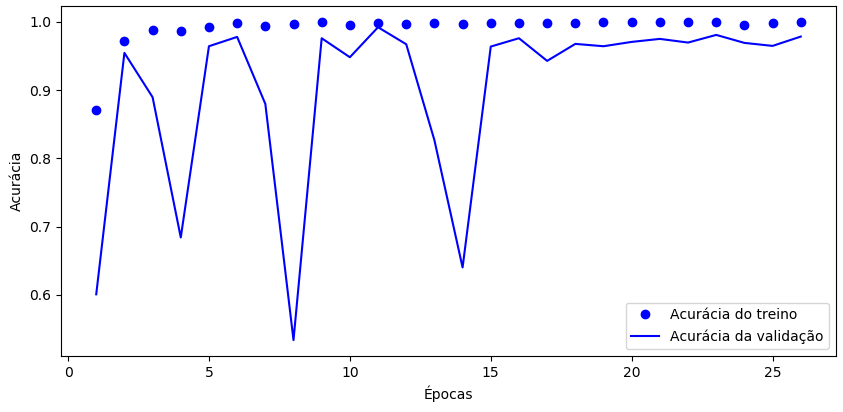
\includegraphics[width=\linewidth]{img/mobilenet-a-acc}%
    \end{subfigure}
    \hspace{1.5cm}
    \begin{subfigure}{0.3\linewidth}
      \caption{\emph{Loss} MobileNet B.\label{subfig:alexnet-b-loss}}
      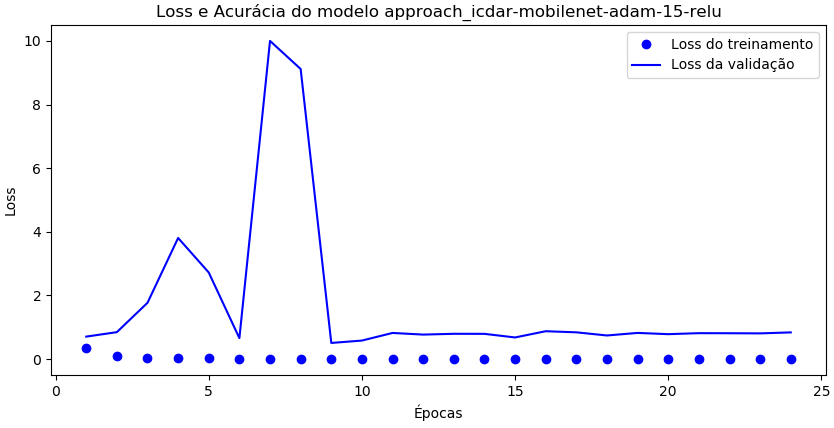
\includegraphics[width=\linewidth]{img/mobilenet-b-loss}%
    \end{subfigure}
    \hspace{1.5cm}
    \begin{subfigure}{0.3\linewidth}
      \caption{Acurácia MobileNet B.\label{subfig:alexnet-b-acc}}
      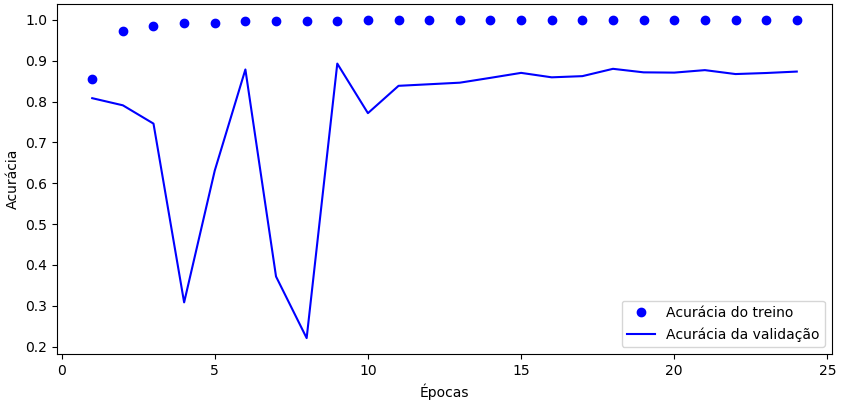
\includegraphics[width=\linewidth]{img/mobilenet-b-acc}%
    \end{subfigure}
    \label{fig:treinamento-alexnet}
  \end{figure}
\end{frame}

\begin{frame}{MobileNet}
  \vskip1\baselineskip
  \begin{figure}[ht!]
    \caption{Matrizes de confusão dos melhores modelos obtidos com a arquitetura MobileNet.}\label{fig:matrizes-lenet}
    \begin{subfigure}{0.4\linewidth}
      \caption{MobileNet A}
      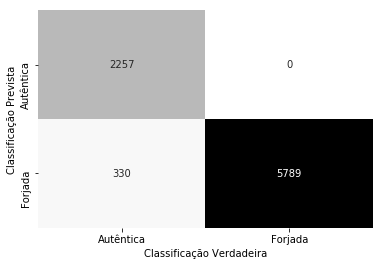
\includegraphics[width=\linewidth]{img/matriz-mobilenet-a}
    \end{subfigure}
    \hspace{2cm}
    \begin{subfigure}{0.4\linewidth}
      \caption{MobileNet B}
      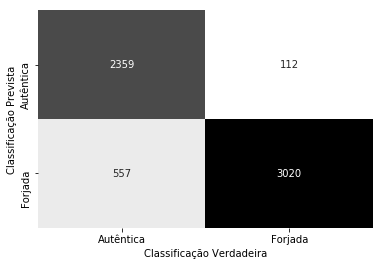
\includegraphics[width=\linewidth]{img/matriz-mobilenet-b}%
    \end{subfigure}
\end{figure}
\end{frame}

\begin{frame}{ShuffleNet}

  \begin{table}[h!]
    \centering
    \caption{Detalhamento dos modelos obtidos com a arquitetura ShuffleNet para cada uma das abordagens consideradas.}
    \label{tab:shufflenet}
    \resizebox{\textwidth}{!}{\begin{tabular}{ccccccc}
    \toprule
    \textbf{Abordagem} & \textbf{Otimizador} & \textbf{\emph{Patience}}  & \textbf{Função de Ativação} & \textbf{Acurácia} & \textbf{F-Score} & \textbf{EER} \\
    \midrule
    Abordagem A & RMSprop & 15 & ReLU & $0.9404$ & $0.9004$ & $7.5400$ \\
    Abordagem B & RMSprop & 15 & ReLU & $0.8345$ & $0.7705$ & $23.8151$\\
    \bottomrule
    \end{tabular}}
    \end{table}

\end{frame}

\begin{frame}{ShuffleNet}

  \begin{figure}[h!]
    \centering
    \caption{Histórico de \emph{loss} e acurácia durante o treinamento dos modelos obtidos com a arquitetura ShuffleNet.}
    \begin{subfigure}{0.3\linewidth}
      \caption{\emph{Loss} ShuffleNet A.\label{subfig:alexnet-a-loss}}
      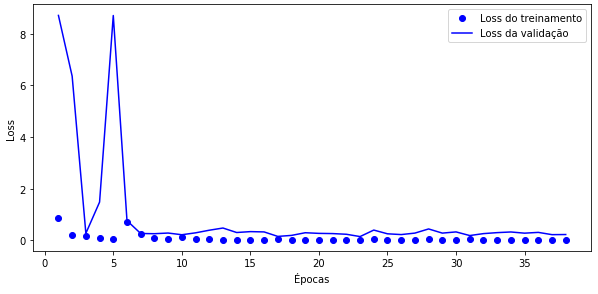
\includegraphics[width=\linewidth]{img/shufflenet-a-loss}%
    \end{subfigure}
    \hspace{1.5cm}
    \begin{subfigure}{0.3\linewidth}
      \caption{Acurácia ShuffleNet A.\label{subfig:alexnet-a-acc}}
      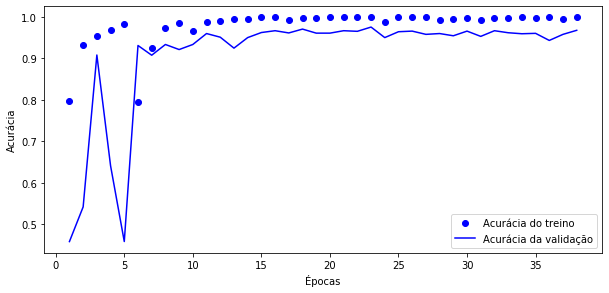
\includegraphics[width=\linewidth]{img/shufflenet-a-acc}%
    \end{subfigure}
    \hspace{1.5cm}
    \begin{subfigure}{0.3\linewidth}
      \caption{\emph{Loss} ShuffleNet B.\label{subfig:alexnet-b-loss}}
      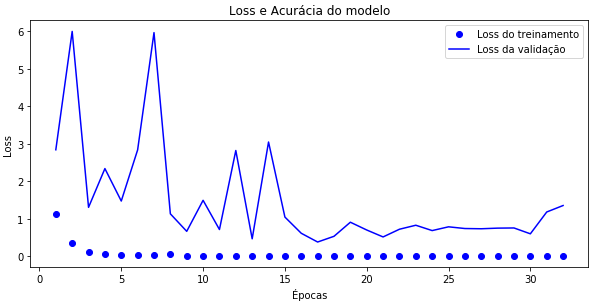
\includegraphics[width=\linewidth]{img/shufflenet-b-loss}%
    \end{subfigure}
    \hspace{1.5cm}
    \begin{subfigure}{0.3\linewidth}
      \caption{Acurácia ShuffleNet B.\label{subfig:alexnet-b-acc}}
      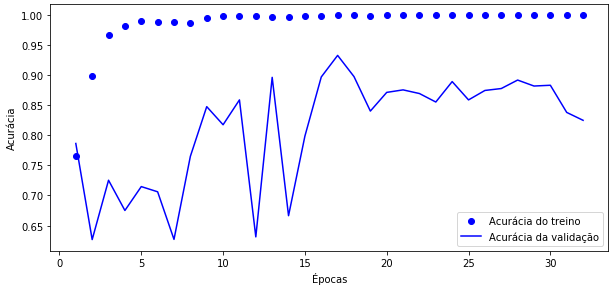
\includegraphics[width=\linewidth]{img/shufflenet-b-acc}%
    \end{subfigure}
    \label{fig:treinamento-alexnet}
  \end{figure}
\end{frame}

\begin{frame}{ShuffleNet}
  \vskip1\baselineskip
  \begin{figure}[ht!]
    \caption{Matrizes de confusão dos modelos obtidos com a arquitetura ShuffleNet.}\label{fig:matrizes-lenet}
    \begin{subfigure}{0.4\linewidth}
      \caption{ShuffleNet A}
      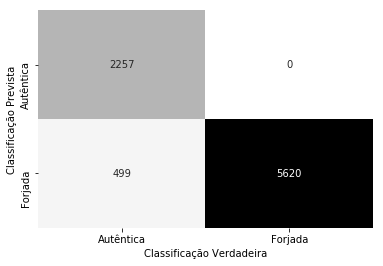
\includegraphics[width=\linewidth]{img/matriz-shufflenet-a}
    \end{subfigure}
    \hspace{2cm}
    \begin{subfigure}{0.4\linewidth}
      \caption{ShuffleNet B}
      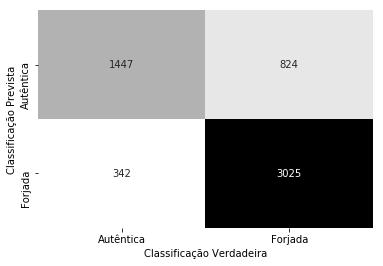
\includegraphics[width=\linewidth]{img/matriz-shufflenet-b}%
    \end{subfigure}
\end{figure}
\end{frame}

\begin{frame}{SqueezeNet}

  \begin{table}[h!]
    \centering
    \caption{Detalhamento dos modelos obtidos com a arquitetura SqueezeNet para cada uma das abordagens consideradas neste trabalho.}
    \label{tab:squeezenet}
    \resizebox{\textwidth}{!}{\begin{tabular}{ccccccc}
    \toprule
    \textbf{Abordagem} & \textbf{Otimizador} & \textbf{\emph{Patience}}  & \textbf{Função de Ativação} & \textbf{Acurácia} & \textbf{F-Score} & \textbf{EER} \\
    \midrule
    Abordagem A & RMSprop & 15 & ReLU & $0.9048$ & $0.8948$ & $11.5074$ \\
    Abordagem B & RMSprop & 15 & ReLU & $0.8210$ & $0.7709$ & $20.1673$\\
    \bottomrule
    \end{tabular}}
    \end{table}

\end{frame}

\begin{frame}{SqueezeNet}

  \begin{figure}[h!]
    \centering
    \caption{Histórico de \emph{loss} e acurácia durante o treinamento dos modelos obtidos com a arquitetura SqueezeNet.}
    \begin{subfigure}{0.3\linewidth}
      \caption{\emph{Loss} SqueezeNet A.\label{subfig:squeezenet-a-loss}}
      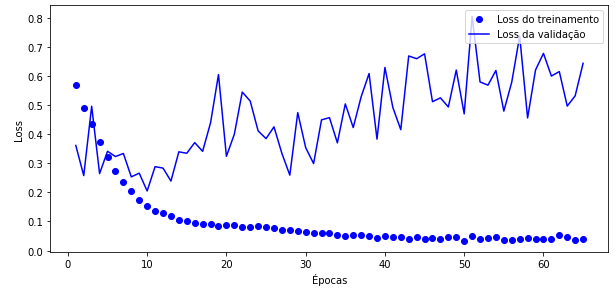
\includegraphics[width=\linewidth]{img/squeezenet-a-loss}%
    \end{subfigure}
    \hspace{1.5cm}
    \begin{subfigure}{0.3\linewidth}
      \caption{Acurácia SqueezeNet A.\label{subfig:squeezenet-a-acc}}
      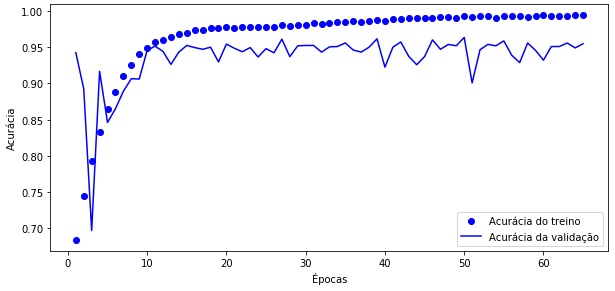
\includegraphics[width=\linewidth]{img/squeezenet-a-acc}%
    \end{subfigure}
    \hspace{1.5cm}
    \begin{subfigure}{0.3\linewidth}
      \caption{\emph{Loss} SqueezeNet B.\label{subfig:squeezenet-b-loss}}
      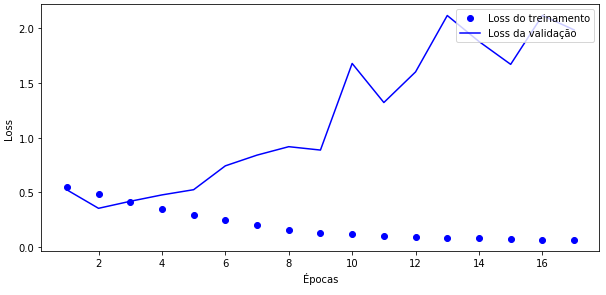
\includegraphics[width=\linewidth]{img/squeezenet-b-loss}%
    \end{subfigure}
    \hspace{1.5cm}
    \begin{subfigure}{0.3\linewidth}
      \caption{Acurácia SqueezeNet B.\label{subfig:squeezenet-b-acc}}
      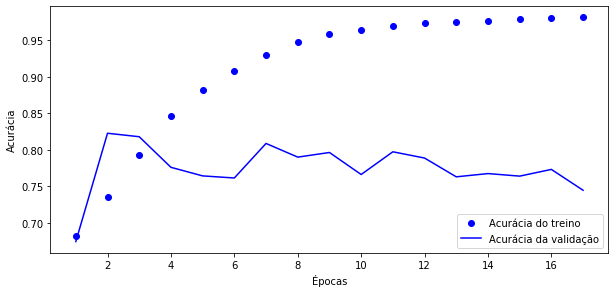
\includegraphics[width=\linewidth]{img/squeezenet-b-acc}%
    \end{subfigure}
    \label{fig:treinamento-alexnet}
  \end{figure}
\end{frame}

\begin{frame}{SqueezeNet}
  \vskip1\baselineskip
  \begin{figure}[ht!]
    \caption{Matrizes de confusão dos modelos obtidos com a arquitetura SqueezeNet.}\label{fig:matrizes-lenet}
    \begin{subfigure}{0.4\linewidth}
      \caption{SqueezeNet A}
      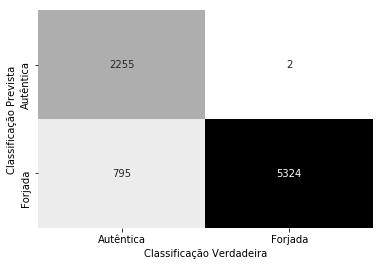
\includegraphics[width=\linewidth]{img/matriz-squeezenet-a}
    \end{subfigure}
    \hspace{2cm}
    \begin{subfigure}{0.4\linewidth}
      \caption{SqueezeNet B}
      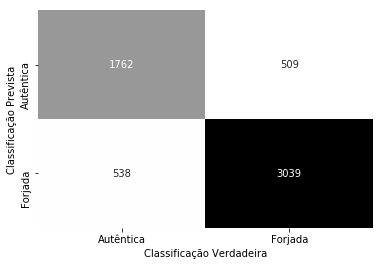
\includegraphics[width=\linewidth]{img/matriz-squeezenet-b}%
    \end{subfigure}
\end{figure}
\end{frame}

\begin{frame}{VGG-16}

  \begin{itemize}
    \item Treinada apenas para abordagem B, com hiperparâmetros \emph{Ad Hoc}
  \end{itemize}

  \begin{table}[h!]
    \centering
    \caption{Detalhamento do modelo obtido com a arquitetura VGG-16 para a abordagem B.}
    \label{tab:vgg}
    \begin{tabular}{cccccc}
    \toprule
    \textbf{Otimizador} & \textbf{\emph{Patience}}  & \textbf{Função de Ativação} & \textbf{Acurácia} & \textbf{F-Score} & \textbf{EER} \\
    \midrule
    RMSprop & 10 & ELU & $0.8391$ & $0.8019$ & $16.1096$ \\
    \bottomrule
    \end{tabular}
    \end{table}

\end{frame}

\begin{frame}{VGG-16}

  \begin{figure}[h!]
    \centering
    \caption{Histórico de \emph{loss} e acurácia durante o treinamento do modelo obtido com a arquitetura VGG-16.}
    \begin{subfigure}{0.44\linewidth}
      \caption{\emph{Loss} VGG-16 B.\label{subfig:squeezenet-b-loss}}
      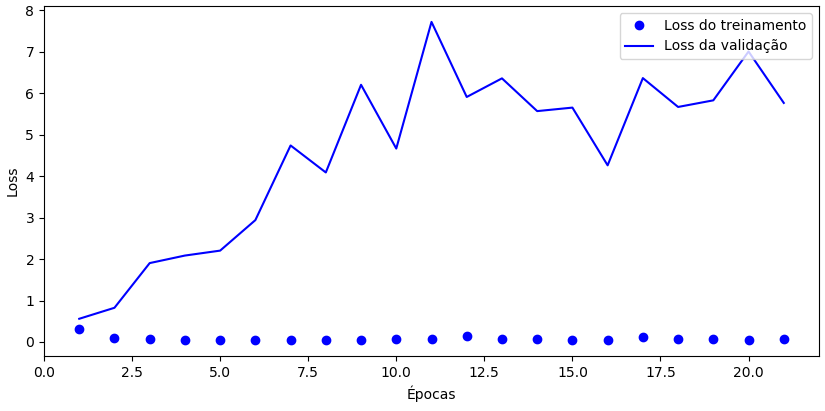
\includegraphics[width=\linewidth]{img/vgg-b-loss}%
    \end{subfigure}
    \hspace{1.5cm}
    \begin{subfigure}{0.44\linewidth}
      \caption{Acurácia VGG-16 B.\label{subfig:squeezenet-b-acc}}
      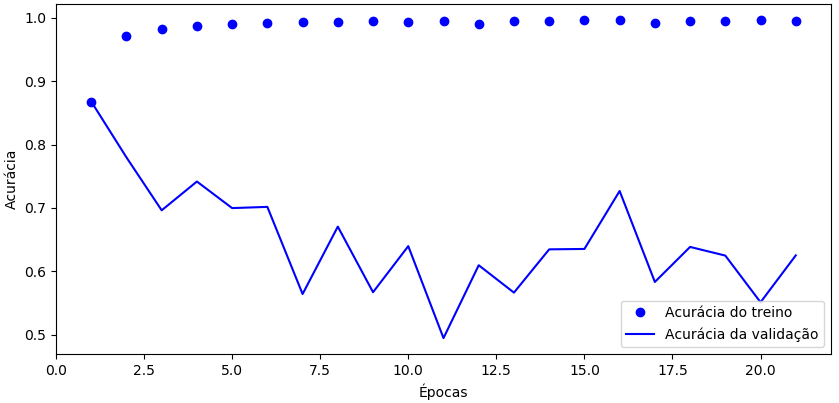
\includegraphics[width=\linewidth]{img/vgg-b-acc}%
    \end{subfigure}
    \label{fig:treinamento-alexnet}
  \end{figure}
\end{frame}

\begin{frame}{VGG-16}
  \vskip1\baselineskip
  \begin{figure}[h]
    \centering
    \caption{Matriz de confusão do modelo obtido com a arquitetura VGG-16.}\label{fig:matrizes-vgg}
    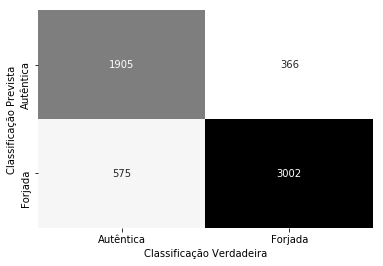
\includegraphics[width=0.6\textwidth]{img/matriz-vgg}
\end{figure}
\end{frame}

\begin{frame}{InceptionV3}

  \begin{itemize}
    \item Treinada apenas para abordagem B, com hiperparâmetros \emph{Ad Hoc}
  \end{itemize}

  \begin{table}[h!]
    \centering
    \caption{Detalhamento do modelo obtido com a arquitetura Inception-V3 para a abordagem B.}
    \label{tab:inception}
    \begin{tabular}{cccccc}
    \toprule
    \textbf{Otimizador} & \textbf{\emph{Patience}}  & \textbf{Função de Ativação} & \textbf{Acurácia} & \textbf{F-Score} & \textbf{EER} \\
    \midrule
    RMSprop & 5 & ELU & $0.8394$ & $0.8070$ & $16.9493$ \\
    \bottomrule
    \end{tabular}
    \end{table}

\end{frame}

\begin{frame}{InceptionV3}

  \begin{figure}[h!]
    \centering
    \caption{Histórico de \emph{loss} e acurácia durante o treinamento do modelo obtido com a arquitetura InceptionV3.}
    \begin{subfigure}{0.44\linewidth}
      \caption{\emph{Loss} InceptionV3 B.\label{subfig:squeezenet-b-loss}}
      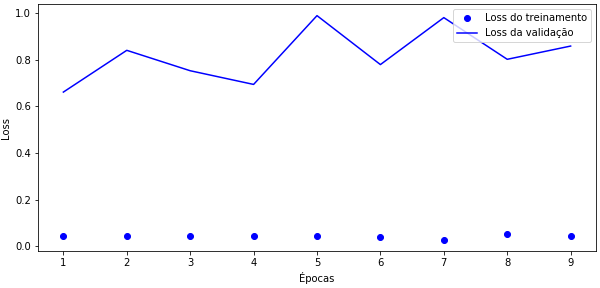
\includegraphics[width=\linewidth]{img/inception-b-loss}%
    \end{subfigure}
    \hspace{1.5cm}
    \begin{subfigure}{0.44\linewidth}
      \caption{Acurácia InceptionV3 B.\label{subfig:squeezenet-b-acc}}
      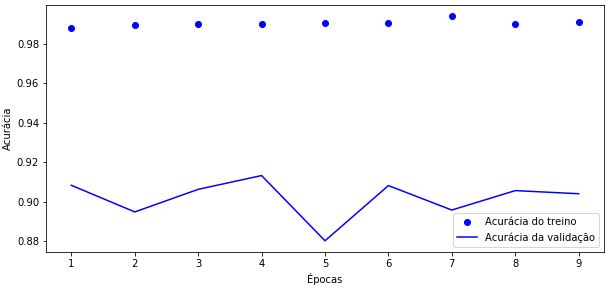
\includegraphics[width=\linewidth]{img/inception-b-acc}%
    \end{subfigure}
    \label{fig:treinamento-alexnet}
  \end{figure}
\end{frame}

\begin{frame}{InceptionV3}
  \vskip1\baselineskip
  \begin{figure}[h]
    \centering
    \caption{Matriz de confusão do modelo obtido com a arquitetura InceptionV3.}\label{fig:matrizes-vgg}
    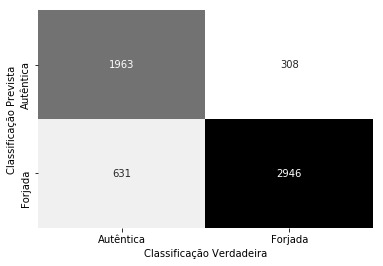
\includegraphics[width=0.6\textwidth]{img/matriz-inception}
\end{figure}
\end{frame}